\section{Performance Evaluation}

We evaluated the performance of our code measuring runtime of our serial and
graph parallel code for a variety of $N$, $M$, and $T$. We generated synthetic
data with random $(A, B, \pi)$ as the true parameters, and initialized our
Baum-Welch training parameters randomly. For both the serial and parallel
versions, we ran 5 update iterations of the Baum-Welch algorithm.  Additionally,
we also varied the number of cores available for Graphlab. R~\cite{r} was used
for data analysis and plotting. 

Our parallel code's runtime, compared to that of the serial version, is shown in
Figure~\ref{fig:runtime-256-500}. We see that, while our GraphLab implementation
runs slower than our serial implementation, the running time still decreases as
we increase the number of processing cores. 

\begin{figure*}[htb]
    \centering
    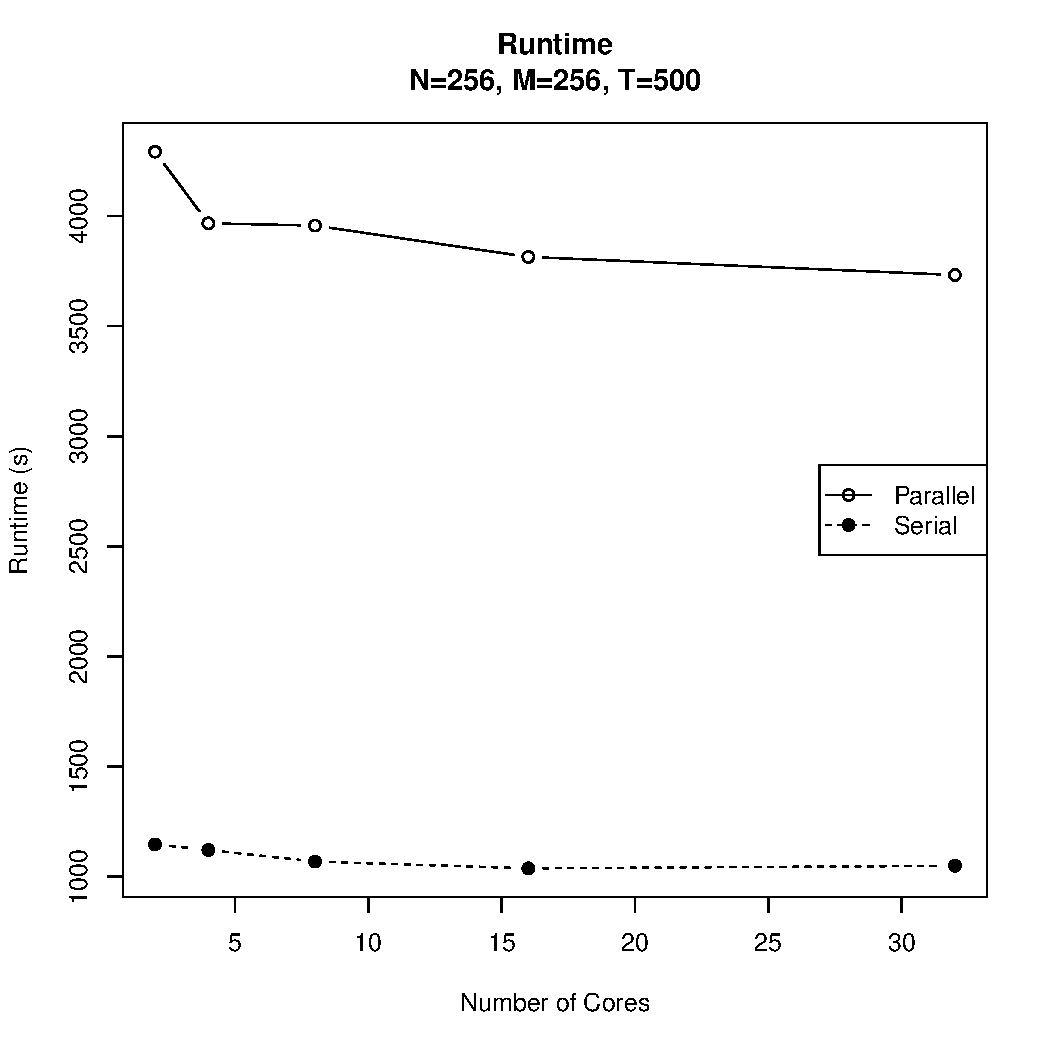
\includegraphics[width=0.6\textwidth]{../figure/runtime-N_256-T_500.pdf}
    \caption{Runtime as a function of number of cores used.}
    \label{fig:runtime-256-500}
\end{figure*}

Figures for other testing conditions are shown in the appendix, in
Figures~\ref{fig:runtime1}--\ref{fig:runtime4}. In general, runtime for the
serial code remains constant, and runtime for the parallel code decreases with
more processors. In many cases, runtime increases when going from 2 to 4
cores---this may represent increased communication cost between more processors.
Noise in our plots may be caused by changes in processing load on the Odyssey
server.

Most compelling, we examined how our implementation scales as we increase the
problem size, especially $N$. A log-log plot of running time vs. $N$ is shown in
Figure~\ref{fig:scaling-16-200}. Judging by the slopes on the graph, our
GraphLab code scales better than the serial code, especially for smaller $N$. 

\begin{figure*}[htb]
    \centering
    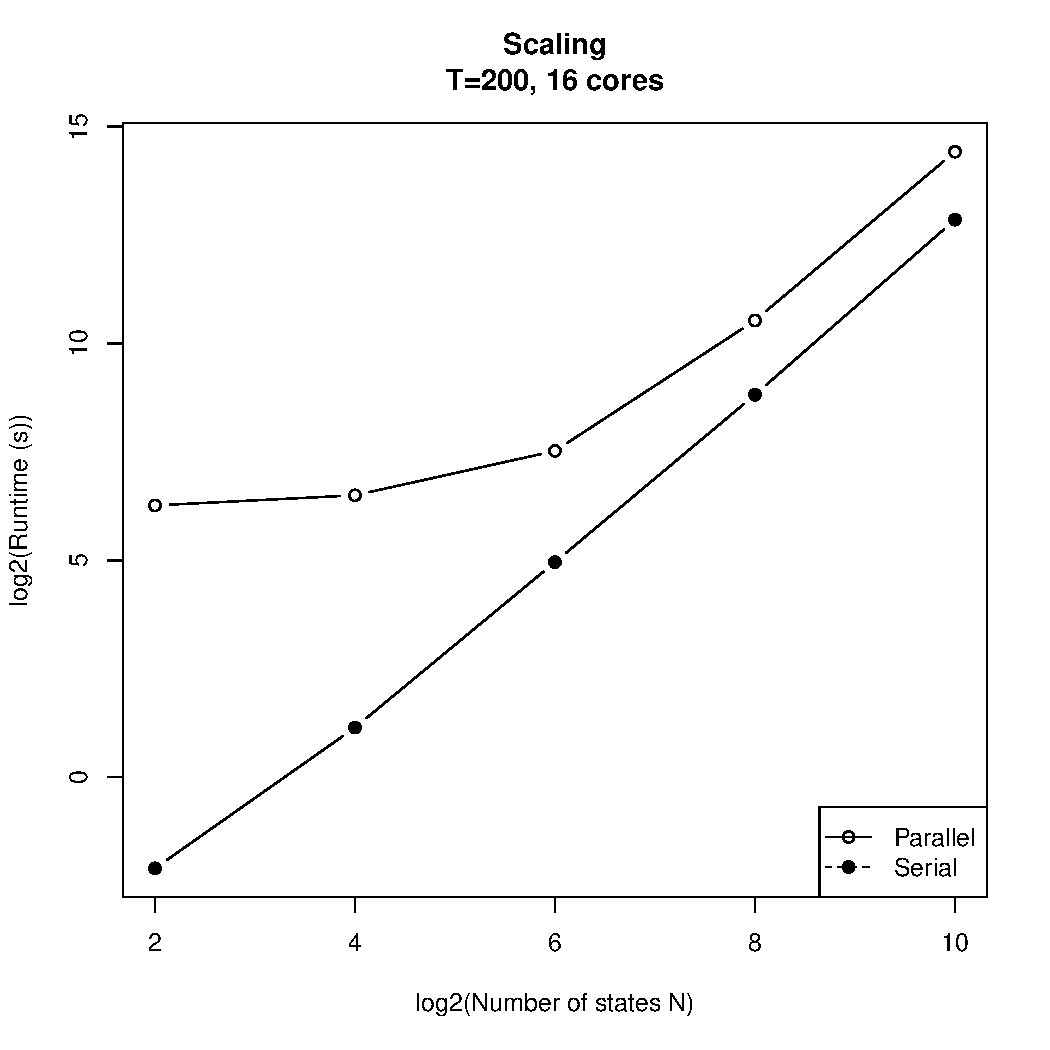
\includegraphics[width=0.6\textwidth]{../figure/scaling-cores_16-T_200.pdf}
    \caption{Log-Log plot of runtime as a function of number of states $N$.}
    \label{fig:scaling-16-200}
\end{figure*}

Additional figures for other testing conditions display similar trends and are
shown in the appendix, Figures~\ref{fig:scaling1}--\ref{fig:scaling4}. 
